\documentclass[a4paper,12pt]{article}

\usepackage[utf8]{inputenc}
\usepackage{graphicx}
\usepackage[table]{xcolor}
\usepackage{pdfpages}
\usepackage{hyperref}
\usepackage{float}
\usepackage[top=1in, bottom=1.25in, left=1in, right=1in]{geometry}
\usepackage{wrapfig}
\usepackage{enumitem}
\usepackage{gensymb}
\usepackage{fancyref}
\usepackage{amssymb}
\usepackage{supertabular}
\usepackage[toc,page]{appendix}

\renewcommand{\familydefault}{\sfdefault}

\definecolor{routinevisualadvisorycolor}{rgb}{0, 1, 0}
\definecolor{nonroutinevisualadvisorycolor}{rgb}{1.0, 0.85, 0}
\definecolor{lightgrey}{rgb}{0.9, 0.9, 0.9}
\definecolor{tablehdrcolor}{rgb}{0.9, 0.9, 1.0}
\definecolor{tablecontcolor}{rgb}{0.95, 0.95, 0.95}
\definecolor{noteboxcolor}{rgb}{.98, 0.8, 0}

\newcommand{\visualadvisory}[2]{%
\colorbox{black}{\makebox[8em]{%
\textcolor{#1visualadvisorycolor}{\large\texttt{#2}}}}%
}

\newcommand{\filetext}[1]{\vspace{.5em}%
\noindent\hspace{0.05\textwidth}\fcolorbox{black}{lightgrey}{%
\parbox{0.9\textwidth}{\texttt{#1}}}%
\vspace{.5em}}

\newcommand{\notebox}[1]{\vspace{.5em}%
\noindent\hspace{0.05\textwidth}\fcolorbox{black}{noteboxcolor}{%
\parbox{0.9\textwidth}{{\large\bf NOTE}\vspace{.35em}\hrule\vspace{.25em}#1}}%
\vspace{.5em}}

\newcommand{\confopt}[1]{\texttt{#1}}

\newcommand{\myfrac}[2]{%
\textsuperscript{#1}\hspace{-0.4em}$\diagup$\hspace{-0.4em}\textsubscript{#2}}

\newcommand{\fileicon}[1]{\raisebox{-.15em}%
{\includegraphics[height=.9em]{../src/#1}}}

\newcommand{\code}[1]{\texttt{#1}}
\newcommand{\dataref}[1]{\texttt{#1}}

\setlist{nolistsep}

\setlength{\abovecaptionskip}{0pt}
\setlength{\belowcaptionskip}{0pt}
\setlength\intextsep{0pt}

\overfullrule=2cm

\title{X-RAAS 2.0 User Manual}
\author{Sašo Kiselkov}


\begin{document}

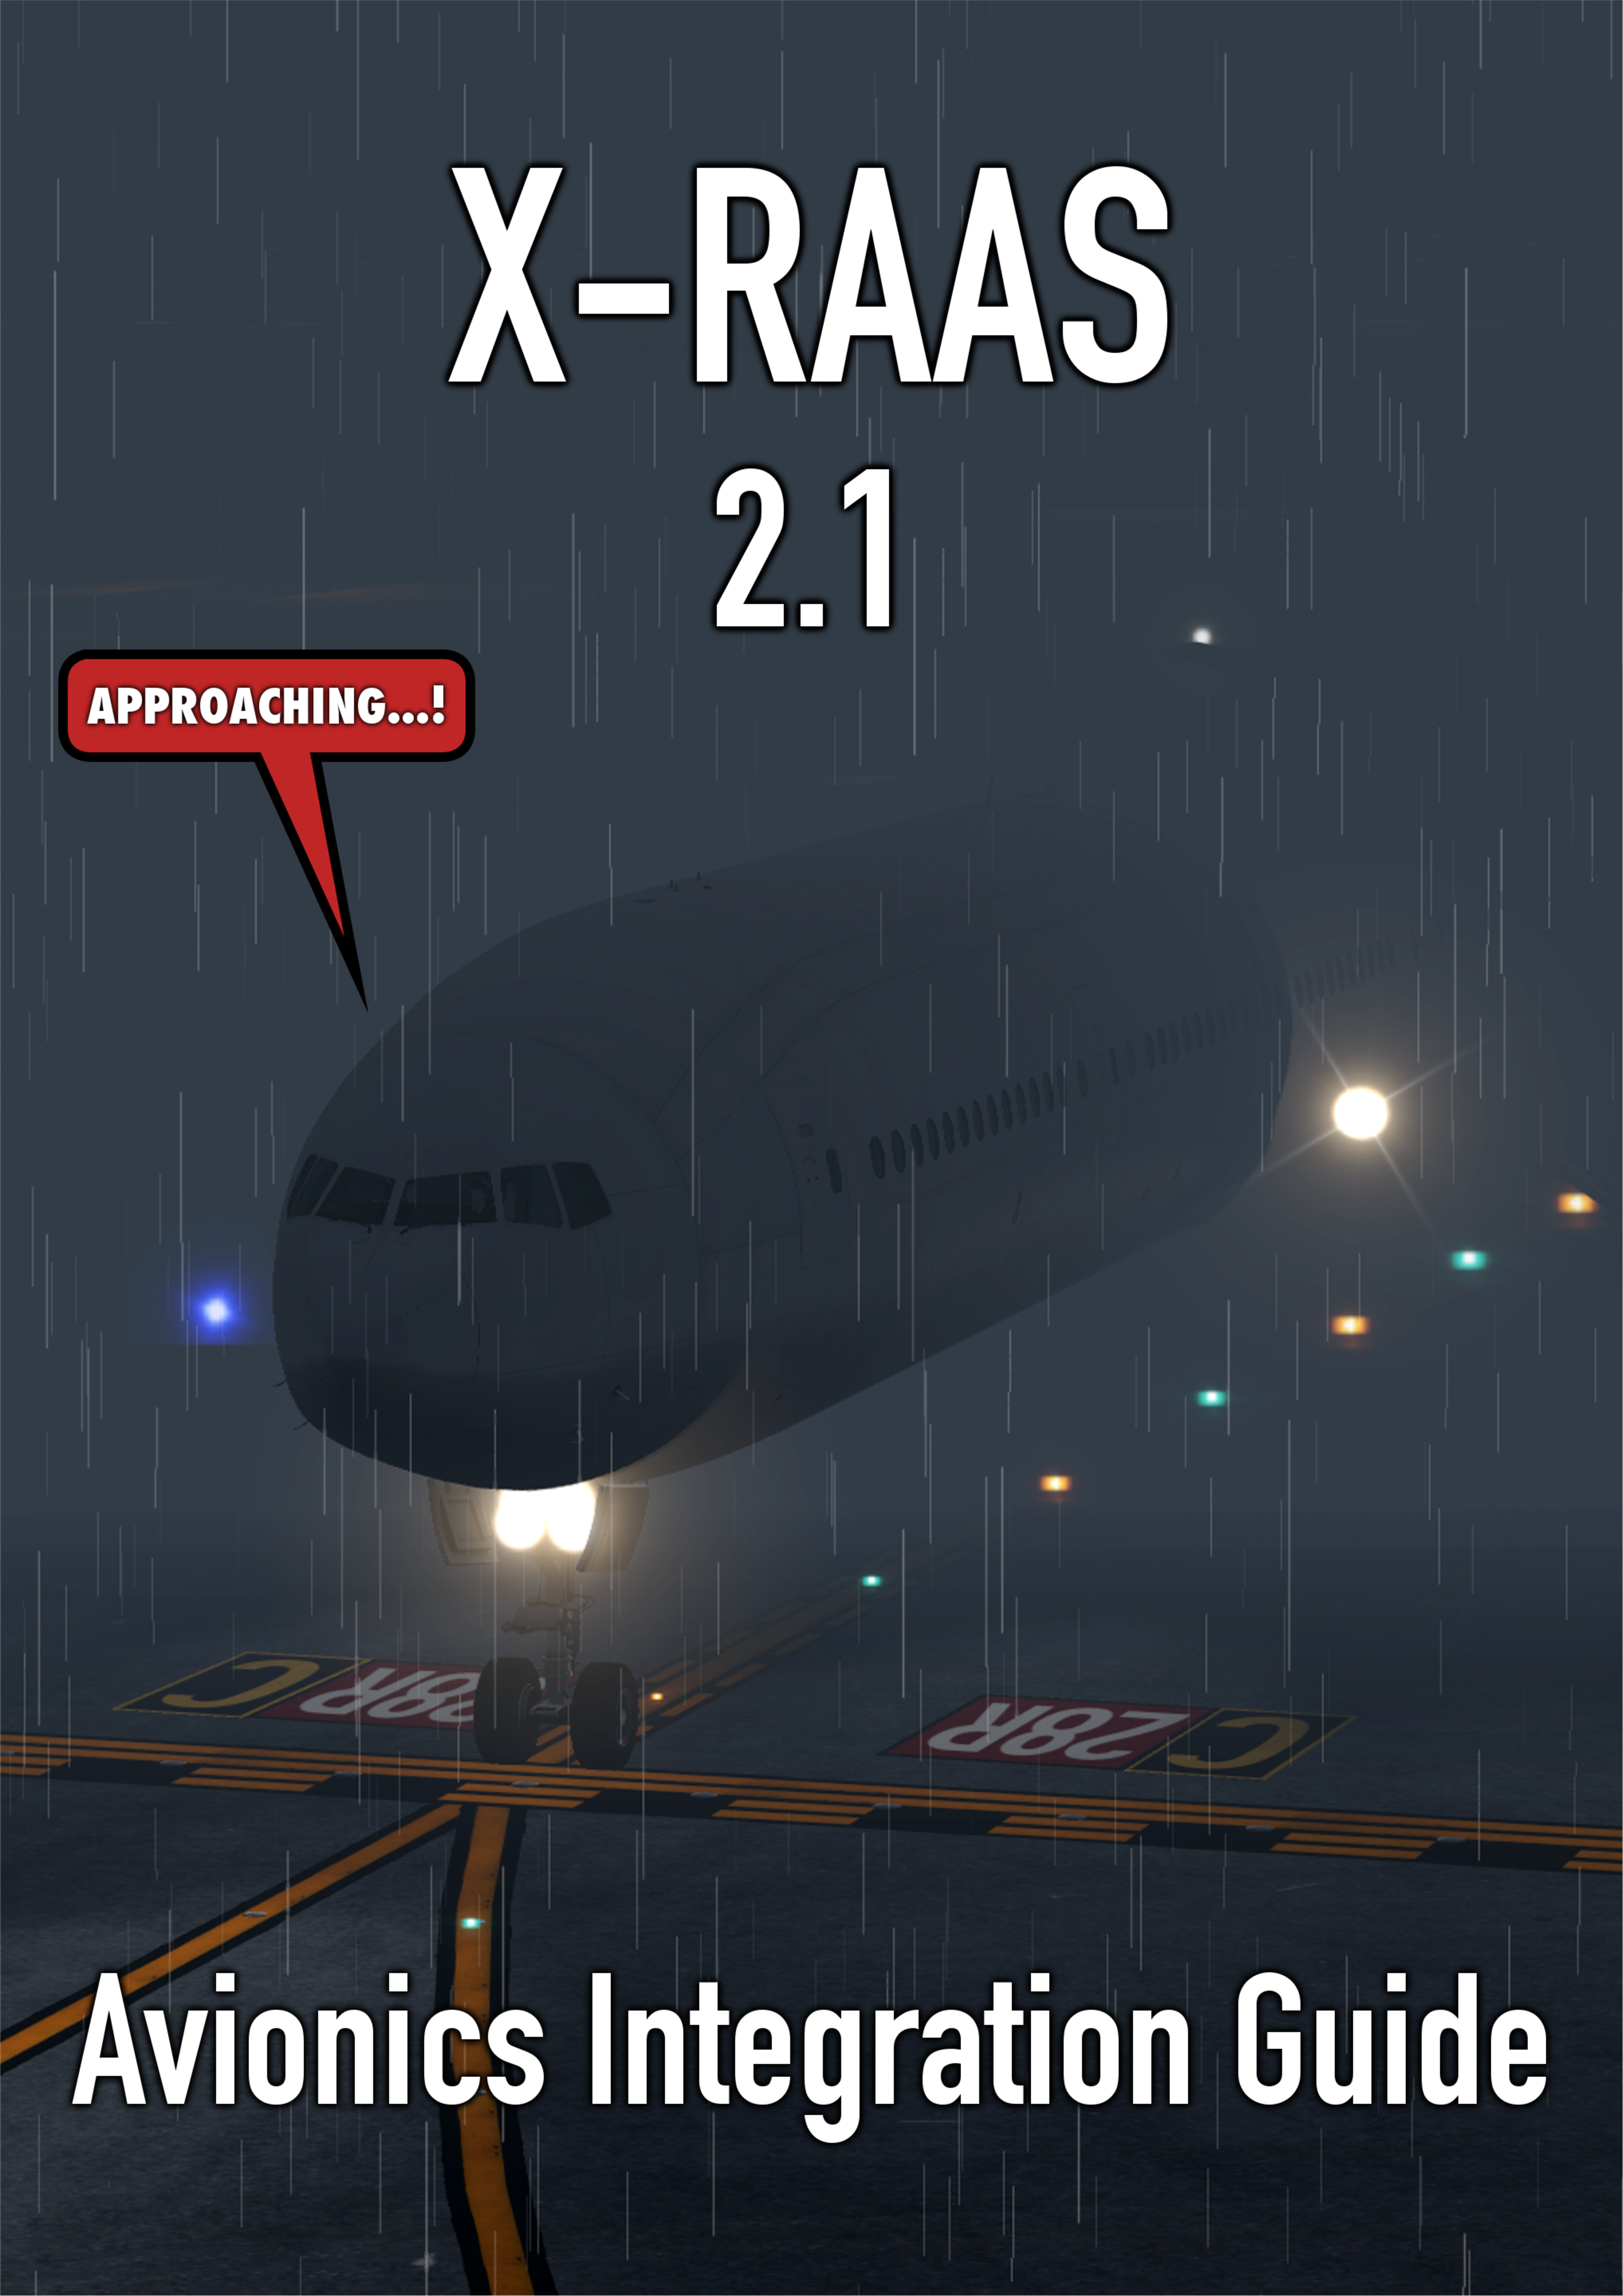
\includepdf{../src/integ_guide_cover.pdf}

\tableofcontents

\newpage

\section{Introduction}

This guide details is meant for aircraft cockpit builders and developers
who wish to integrate X-RAAS into their avionics package. Integration has
many benefits, such as enabling the display of visual alerts on the
aircraft's navigation display in the 3D cockpit and the ability to
control the behavior of the stabilized approach monitor.

X-RAAS can be installed either globally in \texttt{Resources/plugins} or
can be embedded directly in the aircraft model in the plugins subfolder
of that model. See section \ref{sec:Embedding} for more information on
how properly embed X-RAAS. Regardless of the method of delivery, however,
X-RAAS's interface doesn't change.

\section{Receiving visual alert messages}

In many situations, when the plugin generates an aural annunciation, it
can also generate a visual advisory. This is normally meant to be
displayed on the navigation display or a similar such display device in
the cockpit. However, since X-RAAS can't directly paint onto the 3D
cockpit, this needs to be provided by the aircraft's 3D cockpit logic
itself, necessitating this integration. If such integration is not
available (e.g. the aircraft model isn't aware of X-RAAS), X-RAAS
implements a fallback mechanism where the visual alerts are displayed
using an on-screen overlay.

If you choose to provide integration of X-RAAS's visual alerts into your
virtual cockpit logic, you will want to do two things:

\begin{enumerate}

\item Disable the fallback overlay GUI.

\item Receive the alert text to be rendered onto the ND.

\end{enumerate}

\subsection{Disabling the fallback overlay GUI}

For this purpose, all you need to do is write a `1' (or any non-zero
integer value) to the \dataref{xraas/ND\_alert\_overlay\_disabled}
integer dataref. Doing so disables any new messages from being displayed.
Please note that this dataref gets reset back to `0' after each aircraft
unload (i.e.\ in response to \code{XPLM\_MSG\_PLANE\_UNLOADED} when
\code{param == 0}). This is to allow for switching between aircraft which
do and do not want the overlay enabled. You should set it to `1' in your
aircraft avionics loading completion handler. Afterwards, X-RAAS
shouldn't touch it until your aircraft is unloaded again.

\subsection{Receiving the alert text to be displayed}

X-RAAS encodes the string it wants to display into the
\dataref{xraas/ND\_alert} integer dataref using a somewhat non-trivial
format (detailed in appendix \ref{app:EncodingRules}). However, to
facilitate ease of integration, X-RAAS includes sample code in the
\texttt{Documentation/api} folder that helps you with this task. The code
is licensed under the MIT license, giving you maximum freedom in its use,
so you needn't worry about tainting your project with copyleft-licensed
code. The \texttt{api} folder contains implementations in three
languages: C, Lua and Python. If necessary, implementations in other
languages can be provided on request.

The entire API simply consists of one function,
\code{XRAAS\_ND\_msg\_decode}. You pass it the value of the
\code{xraas/ND\_alert} dataref and it returns a string-based
representation of the encoded message, as well as the color code that is
to be applied to the message. For an example of how to use this function,
see the included \texttt{test\_sample} programs in the respective
language subfolders. Alternatively, you can also see how X-RAAS uses it
to render its own fallback overlay in the \code{render\_alert\_texture}
function in \texttt{src/nd\_alert.c} in the X-RAAS source code.

When the ND alert is to be removed from the display, X-RAAS sets
\dataref{xraas/ND\_alert} back to `0'.

\section{GPWS integration}

In the real avionics suite, RAAS is a software function of the EGPWS
computer. As such, the EGPWS can do things such as override or disable
certain or all RAAS annunciations. For X-RAAS, this facility is available
through the following set of datarefs (all datarefs in this table are
integer datarefs):

{\small
\begin{center}

\tablefirsthead{%
\hline
\rowcolor{tablehdrcolor}
\multicolumn{1}{|c}{\textbf{Name}} &
\multicolumn{1}{|c|}{\textbf{Description}} \\
\hline}

\tablehead{%
\hline
\rowcolor{tablecontcolor}
\multicolumn{2}{|l|}{\sl continued from previous page}\\ \hline
\rowcolor{tablehdrcolor}
\multicolumn{1}{|c}{\textbf{Name}} &
\multicolumn{1}{|c|}{\textbf{Description}} \\}

\tabletail{%
\hline
\rowcolor{tablecontcolor}
\multicolumn{2}{|r|}{\sl continued on next page}\\
\hline}

\tablelasttail{\hline}

\begin{supertabular}{|p{0.42\textwidth}|p{0.51\textwidth}|}

\dataref{xraas/override/GPWS\_prio} &
Setting to 1 or 0 enables or disables the use of the
\dataref{xraas/override/GPWS\_prio\_act} dataref. \\

\hline

\dataref{xraas/override/GPWS\_prio\_act} &
Provided the above dataref is set to `1', X-RAAS monitors this dataref to
determine if GPWS callouts currently have priority and consequently if
X-RAAS annunciations should be silenced. You would typically want to set
this dataref to `1' when sounding any GPWS callout such as ``PULL UP!''.\par
As soon as this is set to `1', X-RAAS pauses any currently playing
annunciation and restarts it after the dataref is reset back down to `0'. \\

\hline

\dataref{xraas/override/GPWS\_inop} &
Setting to `1' or `0' enables or disables the use of the
\dataref{xraas/override/GPWS\_inop\_act} dataref. \\

\hline

\dataref{xraas/override/GPWS\_inop\_act} &
Provided the above dataref is set to `1', X-RAAS monitors this dataref to
determine if the GPWS computer is inoperative. This could happen e.g.
during an electrical fault. While set to `1', X-RAAS is inhibited. When
reset back to `0', X-RAAS continues normal operation (assuming sufficient
electrical power). Missed or interrupted annunciations are not replayed,
X-RAAS will behave as if it had been forcibly powered down and back up. \\

\hline

\dataref{xraas/override/GPWS\_flaps\_ovrd} &
Setting to `1' or `0' enables or disables the use of the
\dataref{xraas/override/GPWS\_flaps\_ovrd\_act} dataref. \\

\hline

\dataref{xraas/override/GPWS\_flaps\_ovrd\_act} &
Provided the above dataref is set to `1', X-RAAS monitors this dataref to
determine if the GPWS flaps override mode is active. When the GPWS flaps
override mode is active, all X-RAAS flaps configuration checks are
inhibited. \\

\hline

\dataref{xraas/override/GPWS\_terr\_ovrd} &
Setting to `1' or `0' enables or disables the use of the
\dataref{xraas/override/GPWS\_terr\_ovrd\_act} dataref. \\

\hline

\dataref{xraas/override/GPWS\_terr\_ovrd\_act} &
Provided the above dataref is set to `1', X-RAAS monitors this dataref to
determine if the GPWS terrain override mode is active. When the GPWS
terrain override mode is active, the steep and excessive speed approach
monitors as well as the off-runway landing monitor are inhibited. \\

\end{supertabular}
\end{center}
} % end of \small

\noindent All these datarefs are automatically reset by X-RAAS back to
`0' after an X-RAAS reset (caused by either repositioning the aircraft or
cycling the avionics electrical power), so be sure to set them
periodically if the condition pertaining to a dataref persists.

\section{Approach speed monitor}
\label{EASMon}

During approach, X-RAAS can monitor the aircraft's speed in relation to
its position from the runway threshold and check if the aircraft is
exceeding the pre-determined approach speed set in the FMS at stabilized
approach check gates. To set this approach speed, use the following
integer datarefs:

{\small
\begin{center}

\begin{tabular}{|p{0.42\textwidth}|p{0.51\textwidth}|}

\hline

\rowcolor{tablehdrcolor}
\multicolumn{1}{|c}{\textbf{Name}} &
\multicolumn{1}{|c|}{\textbf{Description}} \\

\hline

\dataref{xraas/override/Vapp} &
Setting to `1' or `0' enables or disables the use of the
\dataref{xraas/override/Vapp\_act} dataref. \\

\hline

\dataref{xraas/override/Vapp\_act} &
Provided the above dataref is set to `1', X-RAAS reads the value of this
dataref to determine the approach speed (V\textsubscript{APP}). Refer to
section 4.14 of the X-RAAS user manual for details on what an approach
speed is. \\

\hline

\dataref{xraas/override/Vref} &
Setting to `1' or `0' enables or disables the use of the
\dataref{xraas/override/Vref\_act} dataref. \\

\hline

\dataref{xraas/override/Vref\_act} &
Provided the above dataref is set to `1', X-RAAS reads the value of this
dataref to determine the reference speed (V\textsubscript{REF}). Refer to
section 4.14 of the X-RAAS user manual for details on what a reference
speed is. \\

\hline

\end{tabular}
\end{center}
} % end of \small

\noindent If both \dataref{Vapp} and \dataref{Vref} are set to `1',
\dataref{Vapp} will be used by the approach speed monitor.

\section{Exact flaps setting checks}

X-RAAS checks flaps settings in two monitors:

\begin{itemize}

\item The on-runway lineup monitor: designed to check that the
appropriate takeoff flaps setting has been made prior to lining up on the
runway. This is to help avoiding triggering the takeoff configuration
warning if the pilots forgot to set the appropriate takeoff flaps setting
and initiate takeoff.

\item The stabilized approach flaps monitor: designed to verify that the
appropriate landing flaps setting is selected at specific altitude gates
on approach. This is to help prevent unstabilized approaches.

\end{itemize}

\noindent The default behavior is to use an upper and lower flaps setting
gate for the takeoff flaps check and only a lower gate for the landing
flaps check. Naturally, these are rather imprecise so as to allow for
meaningful defaults, assuming no tuning for a specific aircraft. However,
if your aircraft simulates an FMS where the flaps setting can be made
explicitly by the pilot1, you can tell X-RAAS \emph{exactly} which flaps
setting it should expect to see in either of these cases, using the
datarefs in the take below. X-RAAS will then issue caution annunciations
if it detects a flaps setting that deviates in any way from the value set
in the datarefs.

{\small
\begin{center}

\begin{tabular}{|p{0.42\textwidth}|p{0.51\textwidth}|}

\hline

\rowcolor{tablehdrcolor}
\multicolumn{1}{|c}{\textbf{Name}} &
\multicolumn{1}{|c|}{\textbf{Description}} \\
\hline

\dataref{xraas/override/takeoff\_flaps} &
Setting to `1' or `0' enables or disables the use of the
xraas/override/takeoff\_flaps\_act dataref. \\

\hline

\dataref{xraas/override/takeoff\_flaps\_act} &
Provided the above dataref is set to `1', X-RAAS reads the value of this
dataref to determine the exact required setting of the
\dataref{sim/flightmodel/controls/flaprqst} dataref which must be set
prior to lining up on the runway. If the actual value of the
\dataref{\ldots/flaprqst} dataref differs by more than 0.01 from this
dataref's value, X-RAAS will issue a caution advisory on lining up on a
runway for takeoff. \\

\hline

\dataref{xraas/override/landing\_flaps} &
Setting to `1' or `0' enables or disables the use of the
\dataref{xraas/override/landing\_flaps\_act} dataref. \\

\hline

\dataref{xraas/override/landing\_flaps\_act} &
Provided the above dataref is set to `1', X-RAAS reads the value of this
dataref to determine the exact required \dataref{\ldots/flaprqst} value
that must be set during approach to a runway. If the actual value of the
\dataref{\ldots/flaprqst} dataref differs by more than 0.01 from this
dataref's value, X-RAAS will issue appropriate advisories during
approach. \\

\hline

\end{tabular}
\end{center}
} % end of \small

\section{Embedding X-RAAS into your aircraft}
\label{sec:Embedding}

While X-RAAS can operate as a stand-alone plugin in the global X-Plane
\texttt{Resources/plugin} folder, embedding X-RAAS into an aircraft model
is a great way to make sure that the RAAS functionality is always
available in a particular aircraft model, no matter the global
environment. To build an embeddable version of X-RAAS, run the following
command in the top level of the X-RAAS source tree:

\filetext{\$ ./build\_release -e}

\noindent The resulting ``X-RAAS2'' folder contains the embeddable
version of the plugin. An embeddable build differs from a stand-alone
build in the following ways:

\begin{enumerate}

\item The plugin signature, name and description are altered to prevent a
conflict and confusion with the globally installed version in the plugin
manager GUI.

\item The embedded plugin automatically disables itself if it detects
that a stand-alone installation of X-RAAS is already present in the
global \texttt{Resources/plugins} folder. This is to prevent duplicate
annunciations and also allows users to upgrade their X-RAAS installation
without having to modify the aircraft model's internal folder layout.

\item An embeddable build doesn't load a global \texttt{X-RAAS.cfg},
since it cannot be invoked when other aircraft are loaded the global
config file shouldn't even be present.

\item The config GUI only allows saving and resetting the configuration
of the aircraft that the plugin is embedded in. Rather than having 4
buttons:

\begin{itemize}

\item SAVE aircraft configuration

\item SAVE global configuration

\item RESET aircraft configuration

\item RESET global configuration

\end{itemize}

The config GUI only shows two buttons (which only operate on the
aircraft-specific configuration):

\begin{itemize}

\item SAVE configuration

\item RESET configuration

\end{itemize}

\item The \texttt{X-RAAS.cache} for caching the airport layouts and
navdata is relocated from the global \texttt{Output/caches/X-RAAS.cache}
into the plugin installation folder itself to avoid polluting the
global simulator environment.

\end{enumerate}

\noindent In terms of interface code, nothing changes between the
stand-alone and embedded version. You should still use the same
interfaces and datarefs described in this guide.

\newpage
\section{About the X-RAAS project}

\subsection{Author}

X-RAAS was written by Sašo Kiselkov. You can contact the author at:

\vspace{1em}

\href{mailto:skiselkov@gmail.com}{skiselkov@gmail.com}

\subsection{License}

X-RAAS is open-source software distributed under the terms of the
\textbf{Common Distribution and Development License}. A copy of the
license text is included in the software package in the \texttt{COPYING}
file. The quick'n'dirty of the terms of this license:

\begin{enumerate}

\item You can copy, modify, run and use X-RAAS in any way you want.

\item You can redistribute your copies (whether modified or not) and even
sell X-RAAS. You can incorporate X-RAAS into your own projects (whether
open-source or not).

\item If you modify X-RAAS and wish to distribute it in any way, you must
share the source code for the modifications you have made to it. If
you've made it part of a larger work, you don't have to share the source
code for all of your work, only the bits of X-RAAS you've modified.

\end{enumerate}

\noindent For the full list of terms, refer to the \texttt{COPYING} file.
An exception to this license are the files under the
\texttt{Documentation/api} folder. These are distributed under the terms
of the MIT License. This pretty much allows you to do whatever you want
with them. The full license text is embedded in the header of each file
under \texttt{api}.

\newpage
\begin{appendix}

\section{Visual alert encoding rules}
\label{app:EncodingRules}

\subsection{Format definition}

This section describes how X-RAAS encodes visual alert messages into the
\dataref{xraas/ND\_alert} dataref. It is mentioned here for completeness
and you are not required to understand the encoding rules unless you plan
on implementing your own decoder.

The message is encoded as a binary integer in native byte order. This is
broken down into multiple bitfields:

{\small
\begin{center}

\tablefirsthead{%
\hline
\rowcolor{tablehdrcolor}
\multicolumn{1}{|c}{\textbf{Bits}} &
\multicolumn{1}{|c|}{\textbf{Description}} \\
\hline}

\tablehead{%
\hline
\rowcolor{tablecontcolor}
\multicolumn{2}{|l|}{\sl continued from previous page}\\ \hline
\rowcolor{tablehdrcolor}
\multicolumn{1}{|c}{\textbf{Bits}} &
\multicolumn{1}{|c|}{\textbf{Description}} \\}

\tabletail{%
\hline
\rowcolor{tablecontcolor}
\multicolumn{2}{|r|}{\sl continued on next page}\\
\hline}

\tablelasttail{\hline}

\begin{supertabular}{|c|p{13.5cm}|}

0 -- 5 &
\textbf{Message type}\newline
Valid values:

\begin{description}

\item[0:] no message present

\item[1:] `FLAPS' message

\item[2:] `TOO HIGH' message

\item[3:] `TOO FAST' message

\item[4:] `UNSTABLE' message

\item[5:] `TAXIWAY' message

\item[6:] `SHORT RUNWAY' message

\item[7:] `ALTM SETTING' message

\item[8:] `APP' message

\item[9:] `ON' message

\item[10:] `LONG LANDING' message

\item[11:] `DEEP LANDING' message

\end{description}

Message types 8 and 9 (`APP' and `ON' messages) also fill the bitfields
for the runway ID, runway ID suffix and distance available. \\

\hline

6 -- 7 &
\textbf{Color}\newline
Valid values:

\begin{description}

\item[0:] message should display in a green color (normal message).

\item[1:] message should display in an amber color (caution message).

\item[2 -- 3:] reserved

\end{description} \\

\hline

8 -- 13 &
\textbf{Runway ID}\newline
Used by message types 8 and 9. Valid values:

\begin{description}

\item[0:] `TAXIWAY'. This is used to signal ``ON TAXIWAY'', by passing
message type 9 and a runway ID of 0.

\item[1 -- 36:] The runway ID for runway `01' through `36'.

\item[37:] ``RWYS'' value. Used when multiple runways are being
approached, e.g. ``APP RWYS'' (message type 8, runway ID 37).

\end{description} \\

\hline

14 -- 15 &
\textbf{Runway ID suffix}\newline
Used by message types 8 and 9. Valid values:

\begin{description}


\item[0:] no suffix. ND should simply show the runway ID, e.g. ``36''.

\item[1:] `RIGHT'. ND should show runway ID with abbreviated suffix, e.g.
``36R''.

\item[2:] `LEFT'. ND should show runway ID with abbreviated suffix, e.g.
``36L''.

\item[3:] `CENTER'. ND should show runway ID with abbreviated suffix,
e.g. ``36C''.

\end{description} \\

\hline

16 -- 23 &
\textbf{Runway length available}\newline
Used by message types 8 and 9. Runway length rounded down to the nearest
100 feet or meters. A value of `0' in this field means `no display'. The
ND should display the value (if non-zero) as a fixed two-digit number
(printf-like format string ``\%02d''). \\

\end{supertabular}
\end{center}
} % end of \small

\newpage
\subsection{Sample message encodings}

{\small
\begin{center}

\begin{tabular}{|p{0.15\textwidth}|p{0.55\textwidth}|c|}

\hline
\rowcolor{tablehdrcolor}
\multicolumn{1}{|c}{\textbf{Dataref value}} &
\multicolumn{1}{|c|}{\textbf{Description}} &
\multicolumn{1}{|c|}{\textbf{ND Display}} \\
\hline

\texttt{0x00000041} &
Amber `FLAPS' message &%
\visualadvisory{nonroutine}{FLAPS}\\

\hline

\texttt{0x00000042} &
Amber `TOO HIGH' message &%
\visualadvisory{nonroutine}{TOO HIGH}\\

\hline

\texttt{0x00000043} &
Amber `TOO FAST' message &%
\visualadvisory{nonroutine}{TOO FAST}\\

\hline

\texttt{0x00000044} &
Amber `UNSTABLE' message &%
\visualadvisory{nonroutine}{UNSTABLE}\\

\hline

\texttt{0x00000045} &
Amber `TAXIWAY' message &%
\visualadvisory{nonroutine}{TAXIWAY}\\

\hline

\texttt{0x00000046} &
Amber `SHORT RUNWAY' message &%
\visualadvisory{nonroutine}{SHORT RUNWAY}\\

\hline

\texttt{0x00000047} &
Amber `ALTM SETTING' message &%
\visualadvisory{nonroutine}{ALTM SETTING}\\

\hline

\texttt{0x00002308} &
Green `APP' message, runway ID \texttt{0x23} (35), runway suffix 0 (`') &%
\visualadvisory{routine}{APP 35}\\

\hline

\texttt{0x00006308} &
Green `APP' message, runway ID \texttt{0x23} (35), runway suffix 1 (`R') &%
\visualadvisory{routine}{APP 35R}\\

\hline

\texttt{0x00002508} &
Green `APP' message, runway ID \texttt{0x25} (37, `RWYS') &%
\visualadvisory{routine}{APP RWYS}\\

\hline

\texttt{0x00142348} &
Amber `APP' message, runway ID \texttt{0x23} (35), runway suffix 0 (`'),
distance available \texttt{0x14} (2000 feet/meters) &%
\visualadvisory{nonroutine}{APP 35 20}\\

\hline

\texttt{0x00086348} &
Amber `APP' message, runway ID \texttt{0x23} (35), runway suffix 1 (`R'),
distance available \texttt{0x08} (800 feet/meters) &%
\visualadvisory{nonroutine}{APP 35R 08}\\

\hline

\texttt{0x00000049} &
Amber `ON' message, runway ID \texttt{0x00} (`TAXIWAY') &%
\visualadvisory{nonroutine}{ON TAXIWAY}\\

\hline

\texttt{0x00002309} &
Green `ON' message, runway ID \texttt{0x23} (35), runway suffix
\texttt{0} (`') &%
\visualadvisory{routine}{ON 35}\\

\hline

\texttt{0x00006309} &
Green `ON' message, runway ID \texttt{0x23} (35), runway suffix
\texttt{1} (`R') &%
\visualadvisory{routine}{ON 35R}\\

\hline

\texttt{0x00002509} &
Green `ON' message, runway ID \texttt{0x25} (37, `RWYS') &%
\visualadvisory{routine}{ON RWYS}\\

\hline

\texttt{0x0014E349} &
Amber `ON' message, runway ID \texttt{0x23} (35), runway suffix
\texttt{3} (`C'), distance available \texttt{0x14} (2000 feet/meters) &%
\visualadvisory{nonroutine}{ON 35C 20}\\

\hline

\texttt{0x0008A349} &
Amber `ON' message, runway ID \texttt{0x23} (35), runway suffix
\texttt{2} (`L'), distance available \texttt{0x08} (800 feet/meters) &%
\visualadvisory{nonroutine}{ON 35L 08}\\

\hline

\texttt{0x0000004A} &
Amber `LONG LANDING' message &%
\visualadvisory{nonroutine}{LONG LANDING}\\

\hline

\texttt{0x0000004B} &
Amber `DEEP LANDING' message &%
\visualadvisory{nonroutine}{DEEP LANDING}\\

\hline

\end{tabular}
\end{center}
} % end of \small

\end{appendix}

\end{document}
